\documentclass[referat]{SCWorks}
\input{preamble.sty}
\setminted{
    frame=lines,
    framesep=2mm,
    baselinestretch=1.2,
    fontsize=\small,
    linenos,
    breaklines
}
\begin{document}
\chair{математической кибернетики и компьютерных наук}
\title{Компьютерный вирус понятие и классификация}
\course{1}
\group{111}
\napravlenie{02.03.02 --- Фундаментальная информатика и информационные технологии}
\studenttitle{студента}
\author{Хохлова Ивана Александровича}
\satitle{доцент, к.\,ф.-м.\,н.}
\chname{С.\,В.\,Миронов}
\satitle{доцент, к.\,ф.-м.\,н.} 
\saname{А.\,С.\,Иванова}
\date{2026}

\secNumbering
\maketitle
\tableofcontents

\intro
Компьютерные вирусы представляют собой одну из наиболее серьёзных угроз информационной безопасности в современном мире. Ежедневно появляются десятки новых вредоносных программ, способных нанести значительный ущерб как отдельным пользователям, так и крупным организациям. Актуальность темы обусловлена необходимостью понимания природы компьютерных вирусов, механизмов их распространения и методов защиты от них.
 
\begin{figure}[h]
    \centering
    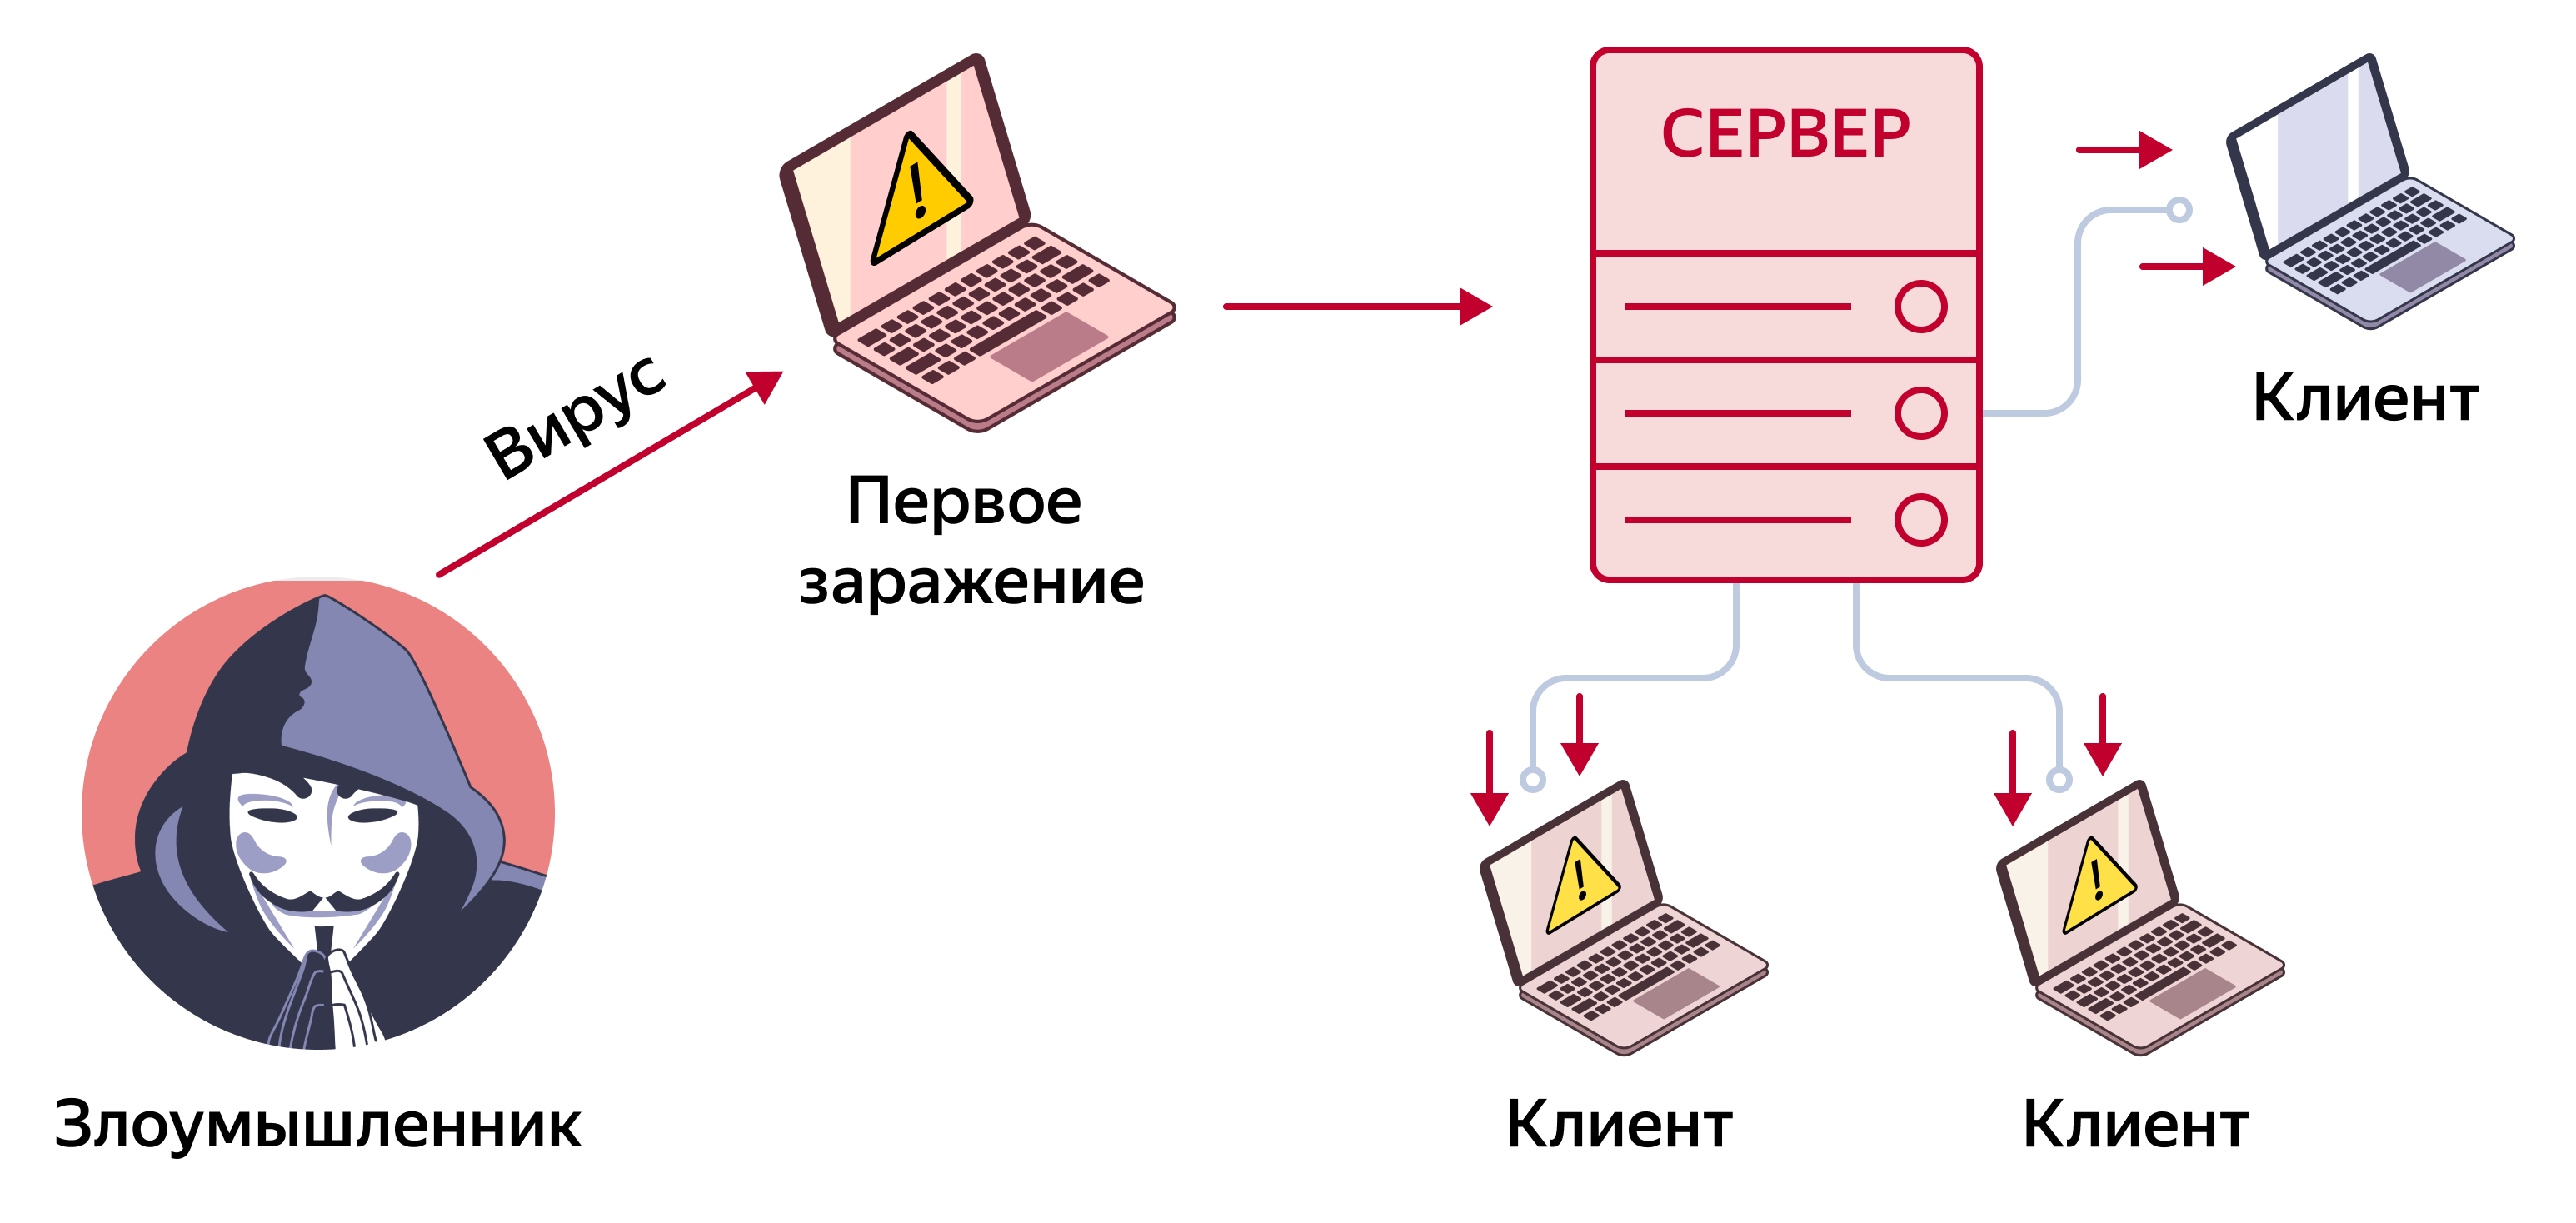
\includegraphics[width=0.5\textwidth]{images/virus_structure.png}
    \caption{Схематичное представление компьютерного вируса}
    \label{fig:virus_structure}
\end{figure}
 
\textbf{Цель} моего реферата --- изучить понятие компьютерного вируса, его классификацию, принципы работы и методы борьбы с ним.
 
Для реализации поставленной цели я ставлю перед собой следующие задачи:
 
\begin{enumerate}
    \item дать определение компьютерного вируса и рассмотреть историю их появления;
    \item изучить классификацию вирусов по различным признакам;
    \item разобрать механизмы работы вирусов на примере загрузочного вируса;
    \item рассмотреть признаки проявления вирусного заражения;
    \item изучить основные типы антивирусных программ и провести обзор современных антивирусных решений.
\end{enumerate}
 
\textbf{Объектом} исследования являются компьютерные вирусы как вредоносные программы, \textbf{предметом} исследования --- классификация вирусов и методы защиты от них.
 
В процессе работы над рефератом применялись анализ литературы, обобщение и систематизация информации.
 
Практическая значимость работы заключается в том, что её материалы могут быть использованы учащимися при изучении информационной безопасности, а также для выбора эффективных средств антивирусной защиты.
\section{Понятие, классификация и принципы работы компьютерных вирусов}
 
\subsection{Определение компьютерного вируса}
 
\textbf{Компьютерный вирус} — это специально написанная, небольшая по размерам программа (т.е. некоторая совокупность выполняемого кода), которая может "приписывать" себя к другим программам ("заражать" их), создавать свои копии и внедрять их в файлы, системные области компьютера и т.д., а также выполнять различные нежелательные действия на компьютере.
 
Программа, внутри которой находится вирус, называется \textbf{заражённой}. Когда такая программа начинает работу, то сначала управление получает вирус. Вирус находит и "заражает" другие программы, а также выполняет какие-нибудь вредные действия (например, портит файлы или таблицу размещения файлов на диске, "засоряет" оперативную память и т.д.). Для маскировки вируса действия по заражению других программ и нанесению вреда могут выполняться не всегда, а, скажем, при выполнении определённых условий.
 
\subsection{Историческая справка}
 
Первые исследования саморазмножающихся искусственных конструкций проводились в середине XX столетия. Термин «компьютерный вирус» появился позднее — официально его автором считается сотрудник Лехайского университета (США) Ф. Коэн в 1984 году на седьмой конференции по безопасности информации.
 
Эксперты считают, что на сегодняшний день число существующих вирусов перевалило за 20 тысяч, причём ежедневно появляется от 6 до 9 новых. «Диких», то есть реально циркулирующих вирусов в настоящее время насчитывается около 260.
 
\begin{figure}[h]
    \centering
    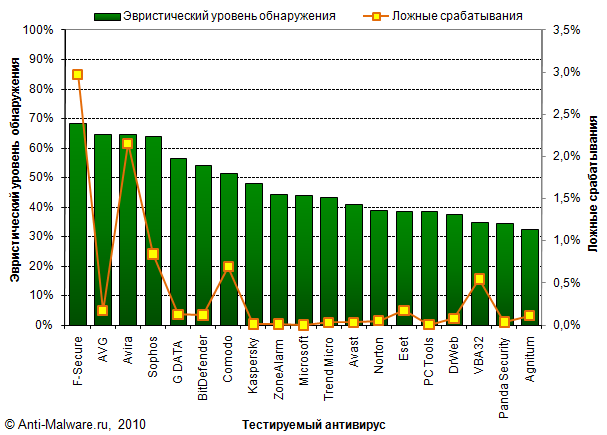
\includegraphics[width=0.7\textwidth]{images/antivirus_comparison.png}
    \caption{Динамика появления новых компьютерных вирусов}
    \label{fig:new_viruses}
\end{figure}
 
\subsection{Классификация компьютерных вирусов}
 
Один из авторитетнейших «вирусологов» страны Евгений Касперский предлагает условно классифицировать вирусы по следующим признакам:
 
\begin{enumerate}
    \item по среде обитания вируса;
    \item по способу заражения среды обитания;
    \item по деструктивным возможностям;
    \item по особенностям алгоритма вируса.
\end{enumerate}
 
\begin{table}[h]
    \centering
    \caption{Классификация компьютерных вирусов по среде обитания}
    \label{tab:classification}
    \begin{tabular}{|c|c|}
        \hline
        \textbf{Тип вируса} & \textbf{Характеристика} \\
        \hline
        Сетевые & Распространяются по компьютерной сети \\
        Файловые & Внедряются в выполняемые файлы \\
        Загрузочные & Внедряются в загрузочный сектор диска (Boot-сектор) \\
        \hline
    \end{tabular}
\end{table}
 
\subsection{Способы заражения}
 
По способу заражения среды обитания вирусы делятся на:
 
\begin{itemize}
    \item \textbf{Резидентные} — находятся в памяти, активны до выключения компьютера;
    \item \textbf{Нерезидентные} — не заражают память, активны ограниченное время.
\end{itemize}
 
\subsection{Деструктивные возможности}
 
По деструктивным возможностям вирусы делятся на:
 
\begin{enumerate}
    \item \textbf{Безвредные} — практически не влияют на работу; уменьшают свободную память на диске в результате своего распространения;
    \item \textbf{Неопасные} — уменьшают свободную память, создают звуковые, графические и прочие эффекты;
    \item \textbf{Опасные} — могут привести к серьёзным сбоям в работе;
    \item \textbf{Очень опасные} — могут привести к потере программ или системных данных.
\end{enumerate}
 
\subsection{Особенности алгоритма вируса}
 
По особенностям алгоритма выделяют следующие типы вирусов:
 
\begin{itemize}
    \item \textbf{Вирусы-«спутники»} — не изменяют файлы, создают для EXE-файлов файлы-спутники с расширением COM;
    \item \textbf{Вирусы-«черви»} — распространяются по сети, рассылают свои копии, вычисляя сетевые адреса;
    \item \textbf{«Паразитические»} — изменяют содержимое дисковых секторов или файлов;
    \item \textbf{«Студенческие»} — примитивны, содержат большое количество ошибок;
    \item \textbf{«Стелс»-вирусы (невидимки)} — перехватывают обращения DOS к поражённым файлам или секторам и подставляют вместо себя незаражённые участки;
    \item \textbf{Вирусы-призраки} — не имеют ни одного постоянного участка кода, труднообнаруживаемы, основное тело вируса зашифровано;
    \item \textbf{Макровирусы} — пишутся не в машинных кодах, а на WordBasic, живут в документах Word.
\end{itemize}
 
\subsection{Как работает вирус: схема функционирования загрузочного вируса}
 
Рассмотрим схему функционирования простого загрузочного вируса, заражающего дискеты. Нормальная схема начальной загрузки выглядит следующим образом:
 
\begin{equation} \label{eq:normal_boot}
    \text{ПНЗ (ПЗУ)} \rightarrow \text{ПНЗ (диск)} \rightarrow \text{СИСТЕМА}
\end{equation}
 
После заражения вирусом в цепочке появляется новое звено:
 
\begin{equation} \label{eq:infected_boot}
    \text{ПНЗ (ПЗУ)} \rightarrow \text{ВИРУС} \rightarrow \text{ПНЗ (диск)} \rightarrow \text{СИСТЕМА}
\end{equation}
 
\begin{figure}[h]
    \centering
    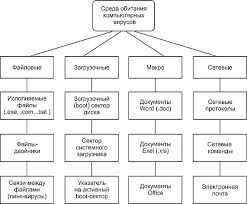
\includegraphics[width=0.6\textwidth]{images/boot_sector.png}
    \caption{Схема заражения загрузочного сектора вирусом}
    \label{fig:boot_sector}
\end{figure}
 
\subsection{Программная реализация: имитация работы вируса}
 
Для демонстрации принципов работы вирусов (в учебных целях) рассмотрим простой скрипт, имитирующий поведение вируса:
 
\begin{listing}[h]
\caption{Имитация поведения вируса на Python}
\label{code:virus_simulation}
 
\begin{minted}[frame=lines,linenos]{python}
class VirusSimulation:
    """Учебная имитация поведения компьютерного вируса"""
    
    def __init__(self, name, destructive_power):
        self.name = name
        self.destructive_power = destructive_power  # от 0 до 10
        self.infected_files = []
        
    def infect(self, filename):
        """Имитация заражения файла"""
        if filename not in self.infected_files:
            self.infected_files.append(filename)
            print(f"Вирус {self.name} заразил файл {filename}")
            return True
        return False
    
    def execute_payload(self, condition):
        """Выполнение вредоносных действий при условии"""
        if condition:
            damage = self.destructive_power * 10
            print(f"Активация вируса! Урон: {damage}%")
            return damage
        return 0
    
    def replicate(self):
        """Имитация размножения"""
        print(f"Вирус {self.name} создал копию себя")
        return VirusSimulation(f"{self.name}_copy", self.destructive_power)
 
# Пример использования
virus = VirusSimulation("TestVirus", 7)
virus.infect("program.exe")
virus.infect("program.exe")  # Повторное заражение не происходит
virus.execute_payload(True)
virus.replicate()
\end{minted}
\end{listing}
\section{Антивирусные программы и методы защиты}
 
\subsection{Определение антивирусных программ}
 
Для обнаружения, удаления и защиты от компьютерных вирусов разработаны специальные программы, которые позволяют обнаруживать и уничтожать вирусы. Такие программы называются \textbf{антивирусными}. Современные антивирусные программы представляют собой многофункциональные продукты, сочетающие в себе как превентивные, профилактические средства, так и средства лечения вирусов и восстановления данных.
 
\subsection{Требования к антивирусным программам}
 
Количество и разнообразие вирусов велико, и чтобы их быстро и эффективно обнаружить, антивирусная программа должна отвечать некоторым параметрам.
 
\begin{equation} \label{eq:antivirus_quality}
    Q_{\text{AV}} = \frac{V_{\text{detected}}}{V_{\text{total}}} \times \alpha + \frac{U_{\text{updates}}}{U_{\text{required}}} \times \beta - \frac{F_{\text{false}}}{F_{\text{total}}} \times \gamma
\end{equation}
 
где:
\begin{itemize}
    \item \(Q_{\text{AV}}\) — качество антивирусной программы;
    \item \(V_{\text{detected}}\) — количество обнаруживаемых вирусов;
    \item \(V_{\text{total}}\) — общее количество известных вирусов;
    \item \(U_{\text{updates}}\) — частота обновлений;
    \item \(F_{\text{false}}\) — количество ложных срабатываний;
    \item \(\alpha, \beta, \gamma\) — весовые коэффициенты.
\end{itemize}
 
\subsection{Типы антивирусных программ}
 
Антивирусные программы делятся на:
 
\begin{enumerate}
    \item \textbf{Программы-детекторы} — обеспечивают поиск и обнаружение вирусов в оперативной памяти и на внешних носителях;
    \item \textbf{Программы-доктора (фаги)} — не только находят заражённые файлы, но и «лечат» их;
    \item \textbf{Программы-ревизоры} — запоминают исходное состояние программ и системных областей, затем сравнивают текущее состояние с исходным;
    \item \textbf{Программы-фильтры (сторожа)} — небольшие резидентные программы для обнаружения подозрительных действий;
    \item \textbf{Вакцины (иммунизаторы)} — резидентные программы, предотвращающие заражение файлов.
\end{enumerate}
 
\begin{table}[h]
    \centering
    \caption{Сравнительная характеристика типов антивирусных программ}
    \label{tab:antivirus_types}
    \begin{tabular}{|c|c|c|c|}
        \hline
        \textbf{Тип} & \textbf{Функция} & \textbf{Преимущества} & \textbf{Недостатки} \\
        \hline
        Детекторы & Поиск вирусов & Быстродействие & Не лечат файлы \\
        Доктора & Лечение файлов & Полное восстановление & Могут повредить файлы \\
        Ревизоры & Контроль изменений & Надёжность & Не удаляют вирусы \\
        Фильтры & Мониторинг действий & Раннее обнаружение & «Назойливость» \\
        Вакцины & Профилактика & Предотвращение заражения & Только от известных вирусов \\
        \hline
    \end{tabular}
\end{table}
 
\subsection{Краткий обзор антивирусных программ}
 
\subsubsection{Norton AntiVirus}
 
Один из наиболее известных и популярных антивирусов. Процент распознавания вирусов очень высокий (близок к 100\%). В программе используется механизм, позволяющий распознавать новые неизвестные вирусы. Антивирусные базы обновляются очень часто (иногда обновления появляются несколько раз в неделю).
 
\subsubsection{Dr. Web}
 
Популярный отечественный антивирус. Хорошо распознаёт вирусы, но в его базе их гораздо меньше, чем у других антивирусных программ.
 
\subsubsection{Antiviral Toolkit Pro (Лаборатория Касперского)}
 
Этот антивирус признан во всём мире как один из самых надёжных. Несмотря на простоту в использовании, он обладает всем необходимым арсеналом для борьбы с вирусами. Эвристический механизм, избыточное сканирование, сканирование архивов и упакованных файлов — это далеко не полный перечень его возможностей.
 
\subsection{Программная реализация: поиск сигнатур вирусов}
 
Ниже представлен фрагмент кода на Python, имитирующий простейший сигнатурный метод поиска вирусов:
 
\begin{listing}[h]
\caption{Сигнатурный метод обнаружения вирусов}
\label{code:signature_scanner}
 
\begin{minted}[frame=lines,linenos]{python}
import hashlib
import os
 
class SimpleAntivirus:
    """Упрощённая модель сигнатурного антивируса"""
    
    def __init__(self):
        self.signatures = {}  # словарь: MD5 сигнатуры вирусов
        self.virus_names = {}  # словарь: MD5 -> имя вируса
        
    def add_virus_signature(self, file_path, virus_name):
        """Добавление сигнатуры вируса в базу"""
        with open(file_path, 'rb') as f:
            content = f.read()
            md5_hash = hashlib.md5(content).hexdigest()
            self.signatures[md5_hash] = True
            self.virus_names[md5_hash] = virus_name
            print(f"Добавлена сигнатура вируса {virus_name}: {md5_hash}")
    
    def scan_file(self, file_path):
        """Сканирование файла на наличие вирусов"""
        try:
            with open(file_path, 'rb') as f:
                content = f.read()
                md5_hash = hashlib.md5(content).hexdigest()
                
                if md5_hash in self.signatures:
                    return f"ОБНАРУЖЕН ВИРУС: {self.virus_names[md5_hash]}"
                else:
                    return "Файл чист"
        except Exception as e:
            return f"Ошибка сканирования: {e}"
    
    def heuristic_scan(self, code):
        """Эвристическое сканирование (поиск подозрительных паттернов)"""
        suspicious_patterns = [
            b'DeleteFile', b'Format', b'WriteProcessMemory',
            b'CreateRemoteThread', b'RegSetValue'
        ]
        score = 0
        for pattern in suspicious_patterns:
            if pattern.lower() in code.lower():
                score += 20
                print(f"Обнаружен подозрительный паттерн: {pattern}")
        
        if score >= 60:
            return f"ВЫСОКИЙ РИСК: эвристический уровень {score}%"
        elif score >= 30:
            return f"СРЕДНИЙ РИСК: эвристический уровень {score}%"
        else:
            return f"НИЗКИЙ РИСК: эвристический уровень {score}%"
 
# Пример использования
av = SimpleAntivirus()
# av.add_virus_signature("virus_sample.exe", "TestVirus")
result = av.scan_file("clean_file.exe")
print(result)
\end{minted}
\end{listing}
 
\subsection{Пути проникновения вирусов}
 
Основными путями проникновения вирусов в компьютер являются:
 
\begin{enumerate}
    \item съёмные диски (гибкие и лазерные);
    \item компьютерные сети;
    \item электронная почта;
    \item загрузка файлов из интернета.
\end{enumerate}
 
Заражение жёсткого диска вирусами может произойти при загрузке программы с дискеты, содержащей вирус. Такое заражение может быть и случайным, например, если дискету не вынули из дисковода и перезагрузили компьютер.
\conclusion
В ходе работы над рефератом я выполнил следующие задачи:
 
\begin{enumerate}
    \item дал определение компьютерного вируса и рассмотрел историю их появления;
    \item изучил классификацию вирусов по различным признакам: среде обитания, способу заражения, деструктивным возможностям и особенностям алгоритма;
    \item разобрал механизмы работы вирусов на примере загрузочного вируса;
    \item рассмотрел основные признаки проявления вирусного заражения;
    \item изучил основные типы антивирусных программ (детекторы, доктора, ревизоры, фильтры, вакцины) и провёл обзор современных антивирусных решений.
\end{enumerate}
 
\begin{figure}[h]
    \centering
    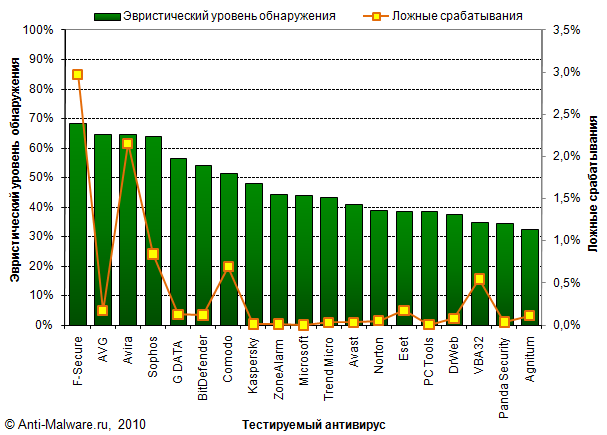
\includegraphics[width=0.6\textwidth]{images/antivirus_comparison.png}
    \caption{Сравнение эффективности антивирусных программ}
    \label{fig:antivirus_comparison}
\end{figure}
 
Несмотря на широкую распространённость антивирусных программ, вирусы продолжают «плодиться». Чтобы справиться с ними, необходимо создавать более универсальные и качественно новые антивирусные программы, которые будут включать в себя все положительные качества своих предшественников.
 
К сожалению, на данный момент нет такой антивирусной программы, которая гарантировала бы защиту от всех разновидностей вирусов на 100\%, но некоторые фирмы, например «Лаборатория Касперского», на сегодняшний день достигли неплохих результатов.
 
Защищённость от вирусов зависит и от грамотности пользователя. Применение вкупе всех видов защит позволит достигнуть высокой безопасности компьютера и, соответственно, информации.

\nocite{*}
\bibliographystyle{ugost2003}
\bibliography{thesis}
\end{document}